\documentclass[a4paper,11pt]{article}
\usepackage[a4,ieis, themeblue]{tuepdfscreen2008}
\usepackage[english]{babel}
\graphicspath{{figures/}}
\usepackage{amsmath,amssymb,amsthm,mathtools,bm,etoolbox, cases, commath}
%\usepackage{mathtime} 
%\setstatustext{Stochastic Operations Research}       % This text is placed in the upper left corner of the poster and can be left empty
%\titlelogo[height=2.8cm]{eurandomlogo}               % You can use this command to insert one logo.

\titleright{\textbf{Operations, Planning, Accounting and Control Group, \\
Department of Industrial Engineering,  
Eindhoven University of Technology, 
The Netherlands
}}      % You can use this commnad INSTEAD OF the \titlelogo command
                                                              % to insert text in the upper right part of the poster (or e.g. multiple logos)


\begin{document}
\begin{slidetop}
\slidetitle[Paul Melkert]{Conditional Correlation Modeling using Machine Learning and Multivariate GARCH}
\begin{multicols}{2}
\section*{Conditional variance-covariance modeling}

We consider a $k$-dimensional log return series, $r_t = (r_{1,t}, \dots, r_{k,t})'$ such that

\begin{align} 
	r_t = H^{1/2}_t z_t, \label{eq:returns_model} \nonumber
\end{align}

where conditional variance-covariances of returns $r_t$ is denoted by a $k\times k$ positive definite matrix $H_t$, with $H_t^{1/2}$ its Cholesky decomposition, and $z_t$ denotes a $k \times 1$ vector of independent and identically distributed random variables with mean zero and unit variance. We consider a reparameterization of $H_t$, i.e. $H_{t}=D_{t}R_{t}D_{t}$, where $D_t$ is a diagonal matrix with conditional volatility of each marginal return series on its diagonal and matrix $R_t$ includes all pairwise correlations $\rho_{i,j,t}$, with $\rho_{i,j,t} = \rho_{j,i,t}$:
 
 
\begin{align} \label{eq:covariance_decomposition} 
	\scalebox{0.78}{
		\begin{pmatrix} h_{1,1,t}^{1/2} &&0 \\ &\ddots \\ 0 &&h_{k,k,t}^{1/2} \end{pmatrix} 
		\begin{pmatrix} 1 &\rho_{1,2,t} &\cdots &\rho_{1,k, t} \\ \rho_{2,1,t} &1 & &\rho_{2,k, t} \\ \vdots &&\ddots &\vdots \\ \rho_{k, 1,t} &\rho_{k, 2,t} &\cdots &1 \end{pmatrix} 
		\begin{pmatrix} h_{1,1,t}^{1/2} &&0 \\ &\ddots \\ 0 &&h_{k,k,t}^{1/2} \end{pmatrix}, \nonumber
		}
\end{align}

Diagonal elements of matrix $D_t$ are modeled parametrically using GARCH(1,1) and GJR-GARCH(1,1) specifications, whereas the conditional correlation matrix $R_t$ is estimated in a nonparametric manner using nonparametric machine learning algorithms k-nearest neighbor and random forest.

 

\bigskip
\iffalse
We consider a wireless link shared by a number of flows. The system operates in a time-slotted fashion, and in each time slot exactly one flow can be scheduled for transmission. The feasible transmission rates for the flows vary over time as a result of fading. In each time slot, a random number of new flows enter the system. Each such flow generates a finite amount of traffic, and exits the system once all its traffic has been processed, see Figure~\ref{fig:overview}.

\begin{center}
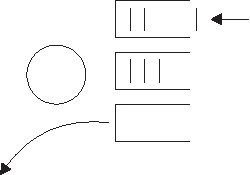
\includegraphics[width=0.6\linewidth]{System_overview}
\figcaption{Overview of the system. \label{fig:overview}}
\end{center}
\fi

The system is a variant of the model considered in Tassiulas and Ephremides~\cite{TE93}\, where it is assumed that the number of flows stays fixed over time, and all flows have a continuous influx of traffic. It can be shown that in this case, so-called {\em MaxWeight} scheduling provides maximum stability, i.e. it achieves stability whenever feasible to do so at all. When using this scheduling rule, in each slot the server selects the flow as follows:

\bigskip 

where $R_i$ denotes the transmission rate, and $Q_i$ denotes the backlog of flow $i$. This is different from MaxRate scheduling for example, where only the transmission rate is used to select the flow to be served.

However, MaxWeight scheduling fails when applied to the dynamic setting under consideration. In contrast to the standard scenario with a fixed number of flows, the instability no longer manifests itself in the form of a few flows with large backlogs, but rather as an excessive number of flows with relatively small backlogs. Because the strategy takes backlog into account, it will give priority to newly arrived flows, so it does not benefit from the service rate variation - the phenomenon that allows the selection of the highest of multiple transmission rates - as it would have when treating all flows equally.

In contrast we consider a strategy close to MaxRate scheduling, and show that this does provide maximum stability. This is done through the Foster-Lyapunov criterion, using the following Lyapunov function:

\bigskip 

where $N_i$ is the number of flows with a backlog of $i$~bits, $B$ denotes the number of bits for each flow, and $R^{\max}$ the maximum feasible transmission rate.

The difference can also be seen in Figure~\ref{fig:graph}, which shows the evolution of the system over time under both strategies.

\begin{center}
\includegraphics[width=\linewidth]{graph_unstable2}
\figcaption{Number of bits in the system plotted against time for MaxWeight and MaxRate scheduling.\label{fig:graph}}
\end{center}

\begin{thebibliography}{99}
\bibitem{TE93}
L. Tassiulas, A. Ephremides (1993).
Dynamic server allocation to parallel queues with randomly varying
connectivity.
{\it IEEE Trans.\ Inf.\ Theory} {\bf 30},
466--478.
\end{thebibliography}
\end{multicols}
\end{slidetop}

\end{document}

